\documentclass[a4paper]{article}

\usepackage[english]{babel}
\usepackage[utf8]{inputenc}
\usepackage{amsmath}
\usepackage{graphicx}
\usepackage{subfigure}
\usepackage[colorinlistoftodos]{todonotes}
\title{Report: An Exploration into Impacts on Network Throughput Brought by Buffer Size Limitation}

\author{Xupeng Wei}

\date{\today}

\begin{document}
\maketitle


\section{Introduction}
\label{sec:introduction}

When we design cross-layer algorithm for network configuration, configuring the network both in short-term time interval and long-term time interval, what we take into consideration in optimization are only link capacities and split ratios, which determine the overall throughput and routing strategies of network. However, buffer size of routers is not referred in our algorithm, which may have impacts on performances of algorithms when buffers are overflow. It is obvious that nothing happens when buffer size is big enough to hold all the requests, but once buffer is filled up by requests, it drops packets, causing a change on traffic characteristic, which makes real traffic condition deviate from our original estimation of network traffic, making performance of algorithm worse. Moreover, different buffer sizes lead to influences on traffic condition in different levels, but configurations derived from optimization have no difference as long as other network conditions remain the same. Therefore, it is significant to examine the impacts brought by buffer, and to find situations under which the cross-layer algorithm is effective, which it is not applicable.

In previous simulation test on TCP cases, we introduced different buffer limitations into each router. Before we introduce buffer limitation into simulation, the performance of cross-layer algorithm is better than rational algorithm which does not take traffic variation into consideration. However, the buffer limitations pull the performance of cross-layer one beneath the rational one, and what is more, the stricter the limitation is, the larger gap between performances for two algorithms is.  This phenomenon indicates that small buffer size can withdraw the superiority of cross-layer algorithm in some cases. Why the cross-layer algorithm performs worse than rational one when suffering a buffer limitation is a problem worthy of consideration, for it can help us to improve cross-layer algorithm to make it more adaptive.
	
Certainly we are able to do simulation with different buffer sizes for our topology with several nodes and dozens of links, but we are not going to do that, because it is really hard to grasp the true mechanism of the cause for worse performance from such a complex system. Thus, we merely put forward some seemly reasonable conjectures from our observations in previous experiments, and test their correctness under some simplified cases.

\section{Conjectures}
\label{sec:conjecture}

The main difference between cross-layer algorithm and rational algorithm is their attitudes toward coming traffic amount and variation. Buffer limitation changes the traffic conditions of network, which makes prediction of both algorithms deviate from real situation, and our cross-layer one suffers more probably because predilections of cross-layer way overstate certain aspects of traffic flow, and correspondingly pay less attention to other ones. Thus, my strategy to find possible explanations is to distinguish the differences of two algorithms, and perform deductions according to these differences to see whether they make sense.
	
One possible speculation is that, the introduction of buffer suppresses the variation of  traffic flow. A router with buffer resembles a funnel with limited volume: if throughput is much more than the amount which container can tolerate, an overflow happens, throwing the surplus part away. As we can see from the phenomena of several simulations done before, the index "time per byte" seems not to converge, which means traffic volume pouring into the network surpasses the capacity of network. Therefore, if we introduce buffers into it, the part of traffic which cannot be processed by routers in time will be trimmed. In this situation, network is like a basin filled with water all the time, with a hole on its bottom. The throughput will maintain unchanged as long as the injection rate is larger than the ejection rate, no matter how fast water is pouring into the basin specifically. Since cross-layer algorithm is designed for the situation which have certain level of traffic variations, it does a good job in variation tolerant, but will does worse in low variation cases -- there is no such thing as a free lunch. Instead, rational approach has a relatively good performance in these low-variation cases.
	
However, the conjecture above has a fatal weakness: although buffer does some trimming jobs, the constant throughput rate is actually brought by low link capacity, not buffer. What buffer do in a congestion traffic condition is to drop packets instead of slowing down the transmission rate. In the TCP cases, traffic condition seems not to change too much, because TCP has a mechanism to retransmit drop packets. In the UDP cases, once packets drop, it will not be transmitted again, and the overall traffic demand decreases. During the process of UDP, traffic variation may become larger because of some unexpected idle period brought by buffer, which is paradoxical to former conjecture.
	
In the following parts, some simple simulations in 2-point UDP case will be performed. The results can give us references and inspirations about the correctness of conjectures, and lead us to further understanding of effects brought by buffer.


\section{Simulation design}
\subsection{Topology}
Instead of considering multi-source and multi-destination cases, the simplest point-to-point case will be used in my simulation, since our goal in this stage is to compare the impacts on performance brought about by buffer and link capacity, instead of judging which optimal algorithm is better. Thus, the concepts of split ratio and seasonal component will not be used in this part. However, it is still necessary to take traffic variation into consideration.
	
Let's start from the most simplest case of simplest cases: point-to-point network topology with pure UDP applications. The network topology is in Figure \ref{fig:topo}.


\begin{figure}
\centering
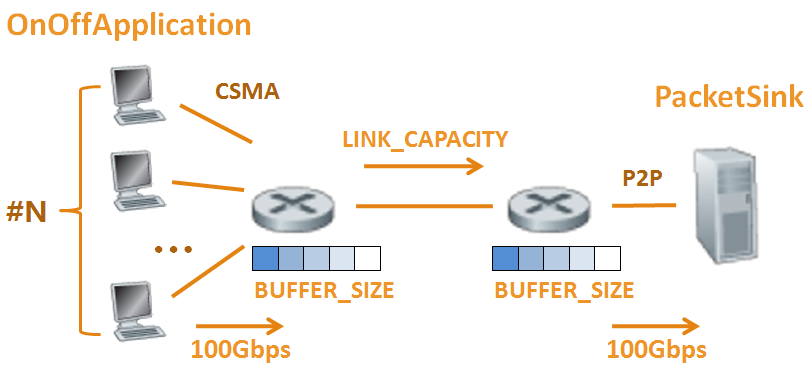
\includegraphics[width=1\textwidth]{topo.png}
\caption{\label{fig:topo}Topology of simulation model.}
\end{figure}

In this topology, varying traffic is generated by several on-off applications. Although it seems that there are multiple senders working together and competing the right to use link between the border router and them, the true story is these applications work in turn. Each of them has its private time slot, and will only be disturbed by its successor because of the mechanism to avoid collision. In spite of the constant sending bit rate of a single on-off application, rates among applications can be different. Therefore, if simulation time is finely cut into several time slots, on-off applications with different bit rates can be adapted in each time slot, and the overall traffic throughput will obey similar distribution with that of the various bit rates.

The following table shows the parameters which is accessible for adjustment.
\newline

// Tunable parameters:

/////////////////////////////////

\#define LINK\_CAPACITY 0.05      // MB/s

\#define TRAFFIC\_INTENSITY 0.12  // MB/s

\#define TRAFFIC\_DEV 0.03        // MB/s

\#define MAX\_SIM\_TIME 3.0        // Seconds

\#define NOISE\_RESOLUTION 0.012  // Seconds

\#define BUFFER\_ON 0             // 1 - On, 0 - Off (Using default settings)

\#define BUFFER\_SIZE 1500        // Bytes

\#define MAX\_PKT\_SIZE 40         // Bytes

/////////////////////////////////
\newline


The inputted traffic for Router Left obeys a Gaussian distribution:

$N$(TRAFFIC\_INTENSITY, TRAFFIC\_DEV{$^2$}).

According to 3-$\sigma$ rule, TRAFFIC\_INTENSITY should be at least 3 times as large as TRAFFIC\_DEV, so that we only gain negative bit rates (which is illegal) with a probability of 0.3\%, which is trivial and is reasonable to be ignored. Please note that although the link transmission rate for CSMA subnet is about 100Gbps, since the applications here are all on-off applications, which must wait for a moment before they begin to send data, and the waiting time is proportional to the size of data. As a result, the rate of data pouring into Router 0 differs from time to time.

Both Router 0 and Router 1 have buffers, but only the buffer on side of Router 0 works, because on Router 1's side, it has an amazingly fast transmission rate, which is able to consume received data almost in a moment.


\subsection{Parameter selection and tuning}
In order to see the effect brought by buffer, we need to know what the performance will be like without a buffer limitation first, and then narrow down buffer size, without changing any other parameters. Theoretically, if the link between two routers has a surfeit of bandwidth, a buffer size which is a little larger than the maximum packet size is enough, because packets is not likely to accumulate in queue. Thus, if we want to see buffer take into effect, the value "LINK\_CAPACITY" should not be set too large. Also, we cannot set "LINK\_CAPACITY" too low; otherwise, the throughput rate of middle link is prone to be a constant, as long as there are some data queuing in the buffer, just like a funnel always having water on its top. Consequently, a link capacity which is slightly bigger than (or near) the average value of traffic intensity is preferable in this case, since it will neither eliminate nor overcast the effect of buffer. This strategy brings limitation to the results of my simulations without doubt, but I haven't caught up other better ideas yet. However, I think there might be some differences in TCP cases, since TCP is a reliable protocol, who has the responsibility to do attempts to deliver packets successfully, behaving differently from UDP.
	
Also, cases with low link capacity and high link capacity will also be included in order to make the results of simulation all-round and confirm my design ideas for simulations. Please note that the strategy above is mostly based on speculations and some qualitative analysis, and the strategy itself needs to be testify in the simulation as well.


\section{Result and mechanism analysis}
\subsection{Validation of noise generation mechanism}
In ns3, sending rates of on-off applications is set before simulations start, and I haven't found a way to make one application generate random traffic requests. Fortunately, we can still use the rectangular input brought by several applications, whose amplitudes are randomly picked obeying Gaussian distribution; then the network can gain a approximate white noise input by putting requests pushed by applications together. However, this mechanism for producing random numbers have two evident drawbacks:

(1) The inputted signal is an approximate Gaussian white noise. In each time slot, the inputted signal remains constant.

(2) Traffic demands are nonnegative, but Gaussian distribution does not have this constraint.


The first drawback is not a big problem. If we divide overall time interval finely into tiny pieces, then we can gain signals whose distribution are quite like Gaussian one. What makes things a little complicated is, CSMA channel has a collision avoidance mechanism, which disturbs the edge characteristic of traffic generation. From the graph of generation rate (Figure \ref{fig:GRV}), we can see that the real-time rate does not seem like a piecewise function as we supposed, and have several high peak, but in this case, we have 250 signal sources, each source will be assigned a 3/250 = 0.012 sec time slot, which is too short for us to distinguish in the graph.

\begin{figure}
\centering
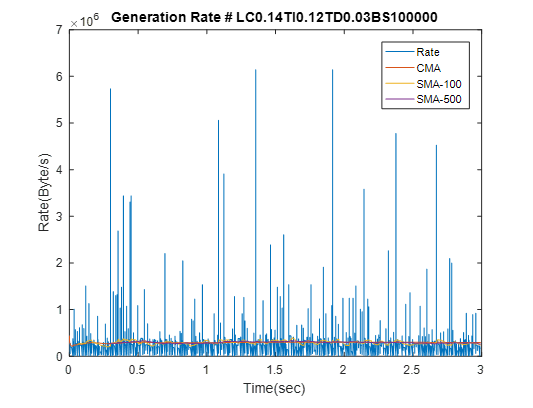
\includegraphics[width=1\textwidth]{GRV.png}
\caption{\label{fig:GRV}Generate Rate for link capacity 0.14MB/s, traffic intensity 0.12MB/s, traffic deviation 0.03MB/s, buffer size 100000. CMA is Cumulative Moving Average, and SMA-X is Simple Moving Average every X packets. SMA is actually an average filter on one-dimension data, and the numbers following "SMA-" is window size of filters.}
\end{figure}


The second drawback tends to increase the real traffic intensity. When I obtain a negative traffic intensity, I will replace it by 1 Byte/s, which makes the beginning part of histogram (see Figure \ref{fig:hist}) look a little taller. The overall average intensity will rise as well. As the overall trend for normal distribution remains, it won't bring many impacts on simulations. Note that the meaning of parameter "traffic intensity" just indicates inputted intensity roughly, instead of show the precise number of average traffic flow.

\begin{figure}
\centering
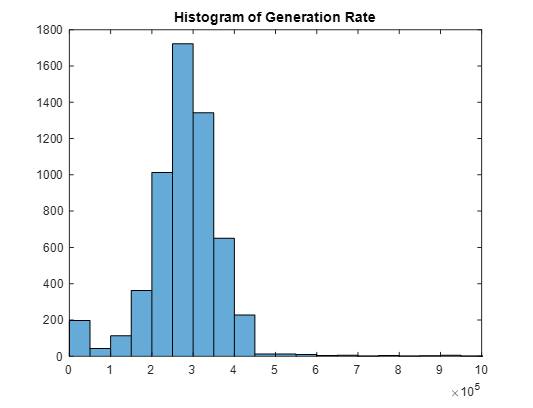
\includegraphics[width=1\textwidth]{hist.png}
\caption{\label{fig:hist}Histogram of Generation Rate.}
\end{figure}

\subsection{Buffer effect on cases with similar link capacity and arrival rate}
\subsubsection{Obtain similar link capacity and arrival rate}
As the effects of buffer are about to be examined, the impacts brought by traffic capacity are expected to be put aside. In previous sections, we discuss what influence on throughput rate will be like if the traffic capacity is too high or too low. In simulation I gain several results to revise the speculations I put forward before, which will be discussed in the following parts. In this part, we just get our feet wet on choosing approximate matched capacity and rate.
	
If link capacity is too low, the throughput side will get saturated. Buffer keeps full almost all the time, and pump out packet with a constant rate. In this case, throughput rate will be a straight line for the most of time, just like Figure \ref{fig:smad}.

\begin{figure}
\centering
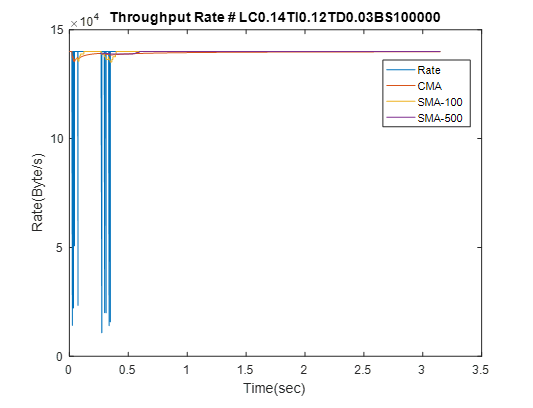
\includegraphics[width=1\textwidth]{smad.png}
\caption{\label{fig:smad} Throughput rate for link capacity 0.14MB/s, traffic intensity 0.12MB/s, traffic deviation 0.03MB/s, buffer size 100,000.}
\end{figure}


If link capacity is too high, the throughput rate will directly reflect the characteristic of arrival traffic, since there is no such a bottleneck link trimming the throughput rate. The curve can have a similar look with inputted signal.

\begin{figure}
\centering
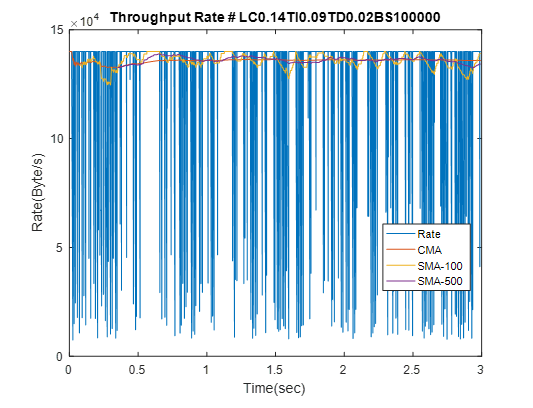
\includegraphics[width=1\textwidth]{smad2.png}
\caption{\label{fig:sd} Throughput rate for link capacity 0.14MB/s, traffic intensity 0.09MB/s, traffic deviation 0.02MB/s, buffer size 100000.}
\end{figure}

In short, the desired look of curve under intensity-rate-matching scenarios is like a piecewise function. In some pieces, throughput rate reaches its upper bound (i.e., link capacity);  in other parts, it looks like Gaussian white noise series, which the inputted signal shape is. Figure \ref{fig:sd} shows such a curve we expected.

\subsubsection{Buffer impacts on throughput intensity and variation}
In intuition, some people tend to have the thought that buffer is a constraint which brings intensive traffic requests into a regular shape, avoiding overload of network, maintaining the stability of flow. The conjecture that buffer lower traffic variation by saturating network volume is based on this belief. However, the experiment results show that this thought is not accurate, and there might be a more complex mechanism leading to a worse performance loss for cross-layer algorithm.
	
I do several simulations under different buffer sizes (Figure \ref{fig:BS1000}-\ref{fig:BS180}), remaining other parameters unchanged. In graphs of throughput rates, we can see that as we lower the buffer size, the time period when throughput rate achieve its upper bound becomes shorter. (Denser the blue lines are, Longer the fluctuation time is, shorter the upper-bound-reaching time is.) What is more, throughput rate changes up and down more frequently under the situation of smaller buffer size. These phenomena are kind of contradictory to our intuition: the introduction of buffer does not bring stability to network system, does not reshape rate curves into more regular ones, but only makes traffic throughput fluctuation more fiercely, even reflects part of the characteristic of inputted white noise signal, which ought to be the things supposed to happen only when link capacity surpasses traffic intensity.

\begin{figure}
\centering
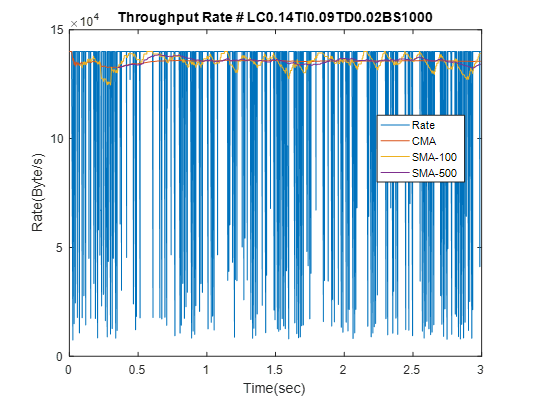
\includegraphics[width=1\textwidth]{BS1000.png}
\caption{\label{fig:BS1000}Throughput rate for Buffer size 1000 }
\end{figure}

\begin{figure}
\centering
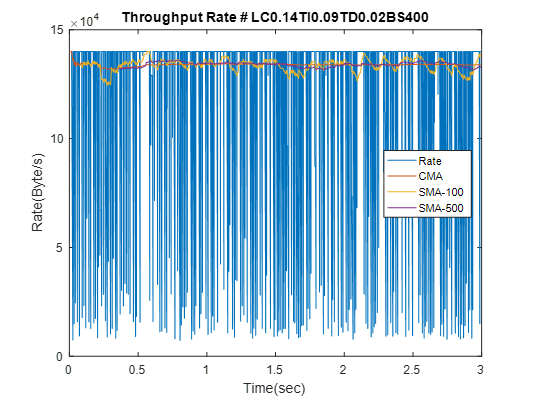
\includegraphics[width=1\textwidth]{BS400.png}
\caption{\label{fig:BS400} Throughput rate for Buffer size 400}
\end{figure}

\begin{figure}
\centering
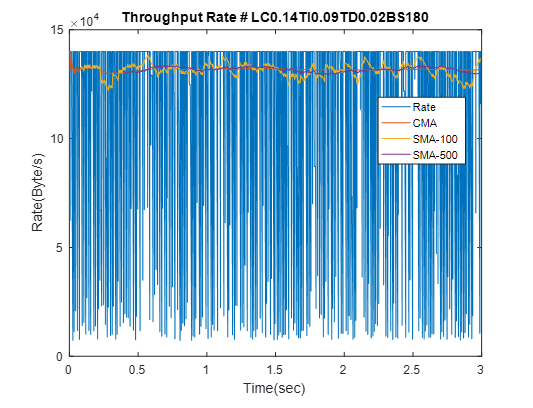
\includegraphics[width=1\textwidth]{BS180.png}
\caption{\label{fig:BS180}Throughput rate for Buffer size 180 }
\end{figure}


	
Why does throughput rate change in such a counterintuitive way? The essential cause is the protocol we use in simulations: UDP. During UDP transmissions, each packet will be sent only once. Thus, the burden of network is eased when packets are dropped. As the traffic demand goes up and down, when buffer size is large enough, the data waiting for transfer keeps rising; when buffer size is limited, it will become a different story. Buffer will trim the traffic demand when it reaches a high level, but network will do nothing to compensate previous packet loss since it adapts UDP protocol, which is not responsible for re-sending data. Thus, when network get into a congestion state, the overall data need to transfer are threw away. When network return to normal burden or a more relaxing state, network with large buffer continues unfinished jobs during this period. However, network with relatively small buffer only does part of it, and soon get into idleness: the loss packets has been threw away and will never come back because UDP protocol of the packets. More packets it drops, longer time network will probably have for idleness.
	
The mechanism above is shown by the simulation results, but it is not easy to see these phenomena directly from real-time throughput ratio, as it keeps fluctuating all the time. Instead, we use moving averages as overall metrics of traffic condition. The function of these moving averages is smoothing, so that the trend of traffic rate can be readable for us. I adapt two kinds of moving averages in analysis. Cumulative moving average is an iterative average which reflects the long term trend of time series, but not accurate in local areas. Simple moving average is a more flexible moving average which can adjust its resolution by tuning the window size. SMA index can preserve part of the information of fluctuation. See results in Figure \ref{fig:CMA}-\ref{fig:SMA500}.

\begin{figure}
\centering
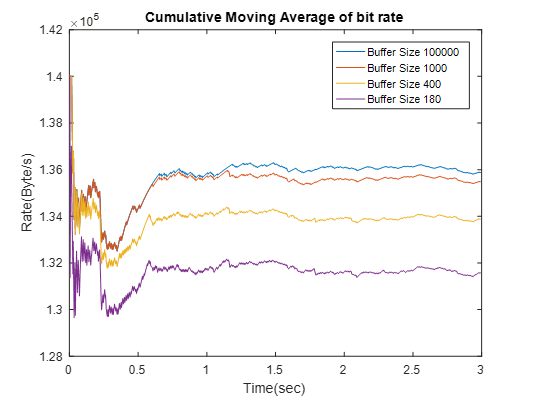
\includegraphics[width=1\textwidth]{CMA.png}
\caption{\label{fig:CMA}Cumulative Moving Average of bit rate }
\end{figure}

\begin{figure}
\centering
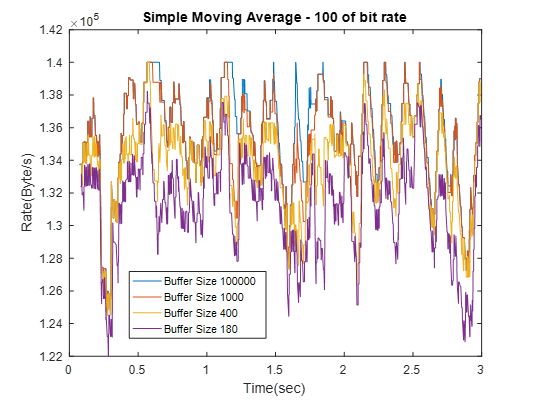
\includegraphics[width=1\textwidth]{SMA100.png}
\caption{\label{fig:SMA100}Simple Moving Average - 100 }
\end{figure}

\begin{figure}
\centering
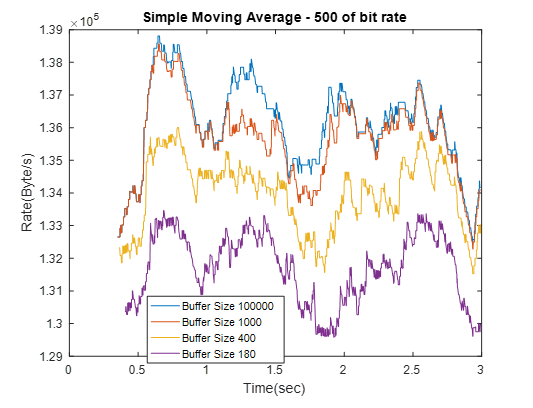
\includegraphics[width=1\textwidth]{SMA500.png}
\caption{\label{fig:SMA500}Simple Moving Average - 500 }
\end{figure}
	
The smoothed indices allows us to compare overall transfer rate for all of these cases. We find that smaller the buffer size is, lower the overall throughput rate will be. It corresponds with the analysis above: limited buffer size make network core throw packets ought to be delivered away, and therefore lower the throughput rate. We can also calculate the change in traffic variation in Table \ref{tab:throughputVar}.

\begin{table}
\centering
\begin{tabular}{l|r}
Buffer Size & Variance \\\hline
10,000 & 4.4570e+08 \\
1,000 & 4.8523e+08 \\
400 & 6.4060e+08\\
180 & 8.3066e+08
\end{tabular}
\caption{\label{tab:throughputVar}Throughput variation.}
\end{table}

	
It shows that smaller buffer brings us a more fierce fluctuation on traffic flows. It can also be explained in terms of mechanism: small buffer size brings more opportunities for network to get into idle states, which are the source of variation under limited link capacity.

\subsection{Buffer effect on cases with extreme difference between link capacity and arrival rate}
Although we have drawn a conclusion about parameter tuning that link capacity and traffic intensity should be matched in our simulations, the experiments with unmatched parameters are still included in this part, because these experiments are helpful to examine whether my idea of simulation design is correct. Moreover, some mechanism will also be reflected in this part of experiments, though they may not be so clear.

\subsubsection{Low link capacity}

In this case, link capacity is only 1/2 of the traffic intensity. (As the traffic intensity is smaller than the real inputted traffic, this link capacity is smaller than 1/2 of inputted traffic.) When the buffer size is big enough, or, there is no buffer limitation, throughput rate is a constant, as we suppose (Figure \ref{fig:sat}). However, when buffer limitation is introduced, throughput rate declines at some of the points (Figure \ref{fig:fluc}). The reason why it happens is probably the same as we discuss in the cases of previous part: buffer throws away some of the packets, bring more chances of getting into idle for network.


\begin{figure}
\centering
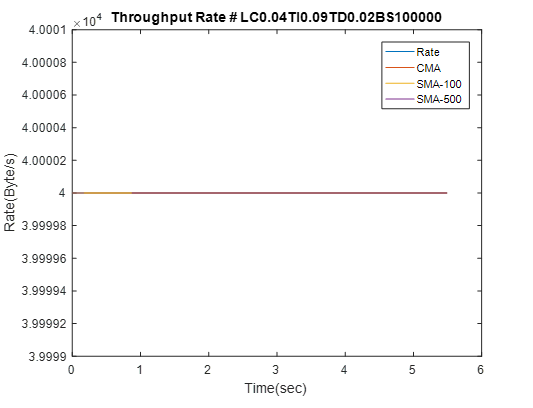
\includegraphics[width=1\textwidth]{sat.png}
\caption{\label{fig:sat}Throughput rate under situation of saturation.}
\end{figure}

\begin{figure}
\centering
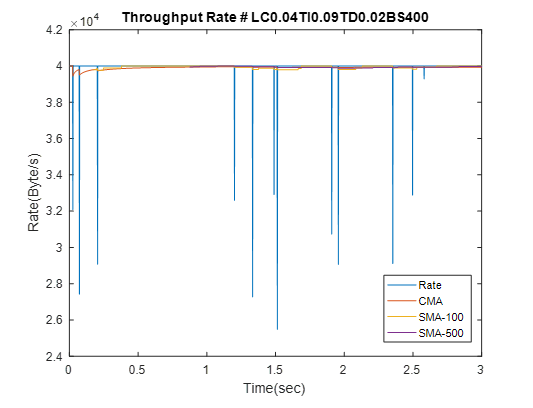
\includegraphics[width=1\textwidth]{fluc.png}
\caption{\label{fig:fluc}Throughput rate under situation of fluctuation.}
\end{figure}

\subsubsection{High link capacity}

The results of this part correspond with exactly what we speculate by intuition. When link capacity is big enough, buffer is short-circuited entirely. The throughput curve is actually the same as the generation curve.(Figure \ref{fig:LC30BS1000}-\ref{fig:LC30BS400})


\begin{figure}
\centering
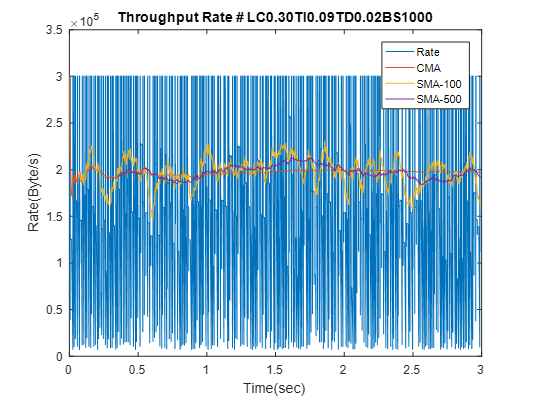
\includegraphics[width=1\textwidth]{LC30BS1000.png}
\caption{\label{fig:LC30BS1000}Throughput rate of high link capacity. (Buffer Size 1000)}
\end{figure}

\begin{figure}
\centering
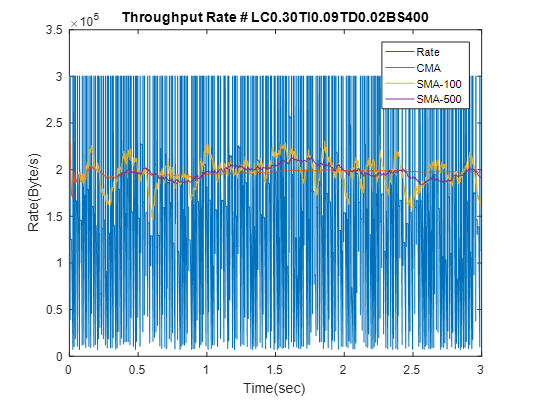
\includegraphics[width=1\textwidth]{LC30BS400.png}
\caption{\label{fig:LC30BS400}Throughput rate of high link capacity. (Buffer Size 400)}
\end{figure}

\newpage
\section{Conclusion}
\label{sec:conclusion}
According to the result of simulations, the cause of worse performance for cross-layer algorithm is not likely to be variation declining caused by buffer limitation, because buffer has two main effects on traffic: lowering overall traffic throughput and intensify traffic variation, instead of trimming traffic variation.  Moreover, buffer will take into effect only when link capacity is close to or lower than intensity of coming traffic. However, the simulations I've done are all under the UDP protocol, which sends each packet only once and does not take responsibility to ensure successful transmissions. Since TCP has a different mechanism, including congestion control, flow control and retransmission, buffer's impacts on traffic flow will interact with these complex mechanism, which makes the traffic characteristic hard to predict. For example, retransmission mechanism supplements traffic requests threw by buffer, making network burden recover to the previous level later. Because of these interactions, although we've gain some useful conclusions from UDP experiments,  I am afraid that this conclusion does not apply for TCP protocol. If we want to see what will happen in TCP cases, one thing we need to think twice is how to tell the effects of buffer from TCP mechanism, which is not easy to distinguish. However, no matter what TCP cases will be like, conclusions about buffer's effect on slightly overloading traffic flow in short time period are likely to be tenable in most of the cases.

\newpage
\begin{thebibliography}{0}

	
	\bibitem{RFC3272} Awduche D, Chiu A, Elwalid A, et al. Overview and Principles of Internet Traffic Engineering[J]. Rfc, 2002, 121(6):239-242.
	\bibitem{SDNchallenge} Hakiri A, Gokhale A, Berthou P, Schmidt DC, Gayraud T. Software-defined networking: Challenges and research opportunities for future internet[J]. Computer Networks, 2014, 75:453-71.
	\bibitem{SDNresCh} Akyildiz I F, Lee A, Wang P, et al. Research challenges for traffic engineering in software defined networks[J]. IEEE Network, 2016, 30(3):52-58.
	\bibitem{responsiveTE} Kandula S, Katabi D, Davie B, et al. Walking the tightrope:responsive yet stable traffic engineering[C]. Conference on Applications. ACM, 2005:253-264.
	\bibitem{preTE} Otoshi T, Ohsita Y, Murata M, et al. Traffic prediction for dynamic traffic engineering[J]. Computer Networks the International Journal of Computer \& Telecommunications Networking, 2015, 85(C):36-50.
	\bibitem{multiRt} Liu X, Mohanraj S, Pioro M, et al. Multipath Routing from a Traffic Engineering Perspective: How Beneficial Is It?[C]. IEEE, International Conference on Network Protocols. IEEE, 2014:143-154.
	\bibitem{trafficMetric} Tune, Paul, and Matthew Roughan. Internet traffic matrices: A primer[J]. Recent Advances in Networking, 2013(1): 1-56.
	\bibitem{bufCore} Wischik D, Mckeown N. Part I:buffer sizes for core routers[J]. Acm Sigcomm Computer Communication Review, 2005, 35(3):75-78.
	\bibitem{bufControl} Towsley D, Towsley D, Wischik D. Part II: control theory for buffer sizing[M]. ACM, 2005.
	
\end{thebibliography}

\end{document}

